


\tikzset{every picture/.style={line width=0.75pt}} %set default line width to 0.75pt        

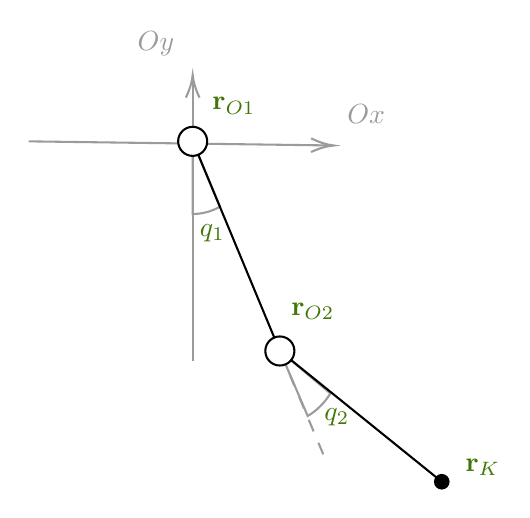
\begin{tikzpicture}[x=0.75pt,y=0.75pt,yscale=-1,xscale=1]
	%uncomment if require: \path (0,300); %set diagram left start at 0, and has height of 300
	
	%Shape: Pie [id:dp044024582329474704] 
	\draw  [color={rgb, 255:red, 155; green, 155; blue, 155 }  ,draw opacity=1 ] (237.35,190.45) .. controls (234.52,195.02) and (230.77,198.77) .. (226.42,201.31) -- (213,170) -- cycle ;
	%Shape: Pie [id:dp8327443137283965] 
	\draw  [color={rgb, 255:red, 155; green, 155; blue, 155 }  ,draw opacity=1 ] (184.19,100.45) .. controls (180.21,102.72) and (175.73,104) .. (171,104) -- (171,69) -- cycle ;
	%Straight Lines [id:da11981673752029831] 
	\draw [color={rgb, 255:red, 155; green, 155; blue, 155 }  ,draw opacity=1 ]   (171,175) -- (171,39) ;
	\draw [shift={(171,37)}, rotate = 90] [color={rgb, 255:red, 155; green, 155; blue, 155 }  ,draw opacity=1 ][line width=0.75]    (10.93,-3.29) .. controls (6.95,-1.4) and (3.31,-0.3) .. (0,0) .. controls (3.31,0.3) and (6.95,1.4) .. (10.93,3.29)   ;
	%Straight Lines [id:da4019711414513023] 
	\draw [color={rgb, 255:red, 155; green, 155; blue, 155 }  ,draw opacity=1 ]   (92,69) -- (237,70.97) ;
	\draw [shift={(239,71)}, rotate = 180.78] [color={rgb, 255:red, 155; green, 155; blue, 155 }  ,draw opacity=1 ][line width=0.75]    (10.93,-3.29) .. controls (6.95,-1.4) and (3.31,-0.3) .. (0,0) .. controls (3.31,0.3) and (6.95,1.4) .. (10.93,3.29)   ;
	%Straight Lines [id:da26868524985077347] 
	\draw    (171,69) -- (213,170) ;
	%Shape: Circle [id:dp05206742113524521] 
	\draw  [fill={rgb, 255:red, 0; green, 0; blue, 0 }  ,fill opacity=1 ] (287.75,233) .. controls (287.75,231.21) and (289.21,229.75) .. (291,229.75) .. controls (292.79,229.75) and (294.25,231.21) .. (294.25,233) .. controls (294.25,234.79) and (292.79,236.25) .. (291,236.25) .. controls (289.21,236.25) and (287.75,234.79) .. (287.75,233) -- cycle ;
	%Shape: Circle [id:dp009854061062177122] 
	\draw  [fill={rgb, 255:red, 255; green, 255; blue, 255 }  ,fill opacity=1 ] (164,69) .. controls (164,65.13) and (167.13,62) .. (171,62) .. controls (174.87,62) and (178,65.13) .. (178,69) .. controls (178,72.87) and (174.87,76) .. (171,76) .. controls (167.13,76) and (164,72.87) .. (164,69) -- cycle ;
	%Straight Lines [id:da271351498464834] 
	\draw    (213,170) -- (291,233) ;
	%Straight Lines [id:da15597835937675186] 
	\draw [color={rgb, 255:red, 155; green, 155; blue, 155 }  ,draw opacity=1 ] [dash pattern={on 4.5pt off 4.5pt}]  (213,170) -- (234,220) ;
	%Shape: Circle [id:dp48139269340211954] 
	\draw  [fill={rgb, 255:red, 255; green, 255; blue, 255 }  ,fill opacity=1 ] (206,170) .. controls (206,166.13) and (209.13,163) .. (213,163) .. controls (216.87,163) and (220,166.13) .. (220,170) .. controls (220,173.87) and (216.87,177) .. (213,177) .. controls (209.13,177) and (206,173.87) .. (206,170) -- cycle ;
	
	% Text Node
	\draw (244,49.73) node [anchor=north west][inner sep=0.75pt]  [color={rgb, 255:red, 155; green, 155; blue, 155 }  ,opacity=1 ]  {$Ox$};
	% Text Node
	\draw (143,14.73) node [anchor=north west][inner sep=0.75pt]  [color={rgb, 255:red, 155; green, 155; blue, 155 }  ,opacity=1 ]  {$Oy$};
	% Text Node
	\draw (301,220.4) node [anchor=north west][inner sep=0.75pt]  [color={rgb, 255:red, 65; green, 117; blue, 5 }  ,opacity=1 ]  {$\mathbf r_{K}$};
	% Text Node
	\draw (179,46.4) node [anchor=north west][inner sep=0.75pt]  [color={rgb, 255:red, 65; green, 117; blue, 5 }  ,opacity=1 ]  {$\mathbf r_{O1}$};
	% Text Node
	\draw (173,107.4) node [anchor=north west][inner sep=0.75pt]  [color={rgb, 255:red, 65; green, 117; blue, 5 }  ,opacity=1 ]  {$q_{1}$};
	% Text Node
	\draw (217,145.4) node [anchor=north west][inner sep=0.75pt]  [color={rgb, 255:red, 65; green, 117; blue, 5 }  ,opacity=1 ]  {$\mathbf r_{O2}$};
	% Text Node
	\draw (233,196.4) node [anchor=north west][inner sep=0.75pt]  [color={rgb, 255:red, 65; green, 117; blue, 5 }  ,opacity=1 ]  {$q_{2}$};
	
	
\end{tikzpicture}